\documentclass{BeamerTemplate}

\usepgfplotslibrary{statistics}
\pgfplotsset{compat=1.17}

% Couleurs des niveaux de facteurs
\definecolor{niv1}{HTML}{000000}
\definecolor{niv2}{HTML}{E41A1C}
\definecolor{niv3}{HTML}{2CA02C}

% Style des graphiques des moyennes (exercices)
\pgfplotsset{
  moyennes/.style={
    width=6.2cm, height=3.9cm,
    xmin=0.7, xmax=3.3, ymin=0, ymax=20,
    xtick={1,2,3}, xticklabels={A1, A2, A3}, ytick={0,5,10,15,20},
    xlabel={Facteur A}, ylabel={Moyenne},
    tick label style={font=\tiny}, label style={font=\scriptsize},
    legend style={font=\tiny, at={(1.02,1)}, anchor=north west},
    legend cell align=left, ymajorgrids, grid style={black!10},
  },
  lB1/.style={niv1, thick, mark=*, mark size=1.5pt},
  lB2/.style={niv2, thick, mark=*, mark size=1.5pt},
  lB3/.style={niv3, thick, mark=*, mark size=1.5pt},
}

\title{Chapitre 5b -- Analyse de la variance à deux facteurs}
\subtitle{STT-1920 Méthodes statistiques}
\date{}

\begin{document}
\begin{frame}[t]
  \titlepage
\end{frame}

\begin{frame}[t]{Plan}
\tableofcontents
\end{frame}

%-------------------------------------------------------------------------------
\section{Expériences factorielles à deux facteurs}
%-------------------------------------------------------------------------------

\begin{frame}[t]{Exemple 1}

On s'intéresse à l'effet de la \alert{température} et de la \alert{concentration}
d'un catalyseur sur le \alert{rendement} d'une réaction chimique, ainsi qu'à leur
\alert{interaction}.

\medskip
On mène une seule expérience où l'on fait varier la température et la
concentration simultanément.

\medskip
\begin{center}
\small
\renewcommand{\arraystretch}{1.3}
\begin{tabular}{c|ccc}
\toprule
 & \multicolumn{3}{c}{Concentration}\\
Température & 0,01 & 0,02 & 0,03\\
\midrule
\multirow{2}{*}{5\,\textdegree C}
  & $Y_{111},Y_{112},Y_{113},$ & $Y_{121},Y_{122},Y_{123},$ & $Y_{131},Y_{132},Y_{133},$\\
  & $Y_{114},Y_{115}$ & $Y_{124},Y_{125}$ & $Y_{134},Y_{135}$\\
\midrule
\multirow{2}{*}{10\,\textdegree C}
  & $Y_{211},Y_{212},Y_{213},$ & $Y_{221},Y_{222},Y_{223},$ & $Y_{231},Y_{232},Y_{233},$\\
  & $Y_{214},Y_{215}$ & $Y_{224},Y_{225}$ & $Y_{234},Y_{235}$\\
\bottomrule
\end{tabular}
\end{center}

\end{frame}

\begin{frame}[t]{Contexte et objectifs}

\begin{itemize}\itemsep3mm
  \item On veut vérifier si l'effet de A dépend du niveau de B, et vice versa:
  \alert{interaction} potentielle entre A et B.
  \item<2-> S'il n'y a pas d'interaction, on pourra estimer ou tester:
  \begin{itemize}
    \item l'effet du facteur A (à $a$ niveaux), et
    \item l'effet du facteur B (à $b$ niveaux).
  \end{itemize}
  \item<3-> On prend $n$ mesures de $Y$ pour chacune des $ab$ combinaisons de
  traitements $\Rightarrow$ $abn$ observations.
  \item<4-> L'assignation des unités aux combinaisons de traitements doit se faire
  de façon \alert{complètement aléatoire}.
\end{itemize}

\end{frame}

\begin{frame}[plain,t]

\centerline{\LARGE\bf\alert{QUIZ !}}

\vspace{3mm}
Dans l'exemple 1,
\begin{itemize}\itemsep4mm
  \item Quels sont les facteurs?
  \item Quelle est la variable réponse?
  \item Que valent $a$, $b$ et $n$?
\end{itemize}
\vspace{3cm}

\end{frame}

%-------------------------------------------------------------------------------
\section{Le modèle}
%-------------------------------------------------------------------------------

\begin{frame}[t]{Le modèle}

\begin{Boite}{{Modèle d'ANOVA, expérience factorielle à deux facteurs}}
\[
Y_{ijk}=\underbrace{\mu+\tau_i+\beta_j+(\tau\beta)_{ij}}_{\mu_{ij}}+\varepsilon_{ijk},
\qquad i=1,\ldots,a;\ j=1,\ldots,b;\ k=1,\ldots,n
\]
\end{Boite}

\small
\begin{itemize}\itemsep0mm
  \item $\mu$ = moyenne globale de la réponse dans la population;
  \item<2-> $\tau_i$ = effet du niveau $i$ du facteur A
  (estimé par $\overline{y}_{i\bullet\bullet}-\overline{y}_{\bullet\bullet\bullet}$);
  \item<3-> $\beta_j$ = effet du niveau $j$ du facteur B
  (estimé par $\overline{y}_{\bullet j\bullet}-\overline{y}_{\bullet\bullet\bullet}$);
  \item<4-> $(\tau\beta)_{ij}$ = effet de l'\alert{interaction} entre A et B au niveau
  $i$ de A et au niveau $j$ de B\\
  (estimé par $\overline{y}_{ij\bullet}-\overline{y}_{i\bullet\bullet}
  -\overline{y}_{\bullet j\bullet}+\overline{y}_{\bullet\bullet\bullet}$);
  \item<5-> $\varepsilon_{ijk}$ = erreurs aléatoires indépendantes de loi $N(0,\sigma^2)$.
\end{itemize}

\end{frame}

\begin{frame}[t]{Les postulats}

Les conditions d'application du modèle à deux facteurs sont les mêmes qu'à
un facteur:

\medskip
\begin{enumerate}\itemsep3mm
  \item les observations $Y_{ijk}$ sont \alert{indépendantes}\\
  \uncover<2->{(donc les erreurs $\varepsilon_{ijk}$ sont indépendantes);}
  \item la \alert{variance} des $Y_{ijk}$ est la même ($\sigma^2$) pour chaque
  combinaison de facteurs\\
  \uncover<3->{(donc la variance des $\varepsilon_{ijk}$ est constante);}
  \item les $Y_{ijk}$ proviennent de lois \alert{normales} $N(\mu_{ij},\sigma^2)$\\
  \uncover<4->{(donc les $\varepsilon_{ijk}$ sont de loi $N(0,\sigma^2)$).}
\end{enumerate}

\end{frame}

\begin{frame}[t]{Graphique des moyennes: illustrer les effets des facteurs}

\begin{center}
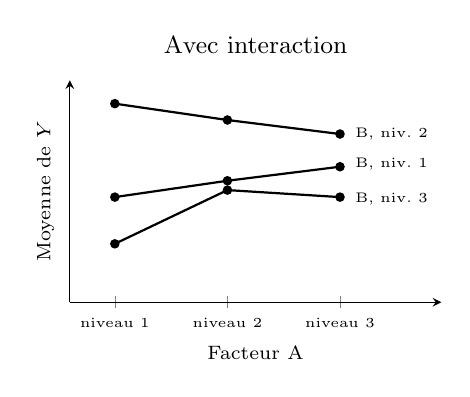
\begin{tikzpicture}
\begin{axis}[width=6.3cm, height=4.4cm, xmin=0.6, xmax=3.9, ymin=0, ymax=9.5,
  axis lines=left, xtick={1,2,3}, xticklabels={niveau 1, niveau 2, niveau 3},
  ytick=\empty, ylabel={Moyenne de $Y$}, xlabel={Facteur A},
  tick label style={font=\tiny}, label style={font=\scriptsize},
  title={Avec interaction}, title style={font=\small}]
  \addplot[black, thick, mark=*, mark size=1.3pt] coordinates {(1,8.5) (2,7.8) (3,7.2)};
  \addplot[black, thick, mark=*, mark size=1.3pt] coordinates {(1,4.5) (2,5.2) (3,5.8)};
  \addplot[black, thick, mark=*, mark size=1.3pt] coordinates {(1,2.5) (2,4.8) (3,4.5)};
  \node[font=\tiny, anchor=west] at (axis cs:3.05,7.2) {B, niv.\ 2};
  \node[font=\tiny, anchor=west] at (axis cs:3.05,5.9) {B, niv.\ 1};
  \node[font=\tiny, anchor=west] at (axis cs:3.05,4.4) {B, niv.\ 3};
\end{axis}
\end{tikzpicture}
\hspace{3mm}
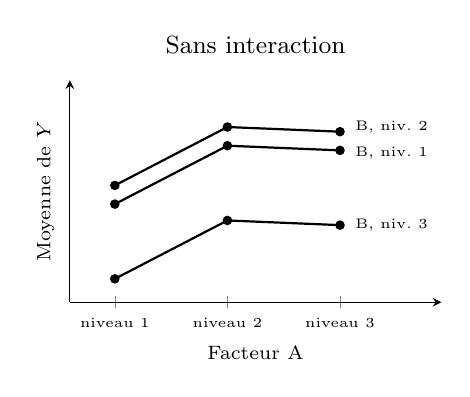
\begin{tikzpicture}
\begin{axis}[width=6.3cm, height=4.4cm, xmin=0.6, xmax=3.9, ymin=0, ymax=9.5,
  axis lines=left, xtick={1,2,3}, xticklabels={niveau 1, niveau 2, niveau 3},
  ytick=\empty, ylabel={Moyenne de $Y$}, xlabel={Facteur A},
  tick label style={font=\tiny}, label style={font=\scriptsize},
  title={Sans interaction}, title style={font=\small}]
  \addplot[black, thick, mark=*, mark size=1.3pt] coordinates {(1,5.0) (2,7.5) (3,7.3)};
  \addplot[black, thick, mark=*, mark size=1.3pt] coordinates {(1,4.2) (2,6.7) (3,6.5)};
  \addplot[black, thick, mark=*, mark size=1.3pt] coordinates {(1,1.0) (2,3.5) (3,3.3)};
  \node[font=\tiny, anchor=west] at (axis cs:3.05,7.5) {B, niv.\ 2};
  \node[font=\tiny, anchor=west] at (axis cs:3.05,6.4) {B, niv.\ 1};
  \node[font=\tiny, anchor=west] at (axis cs:3.05,3.3) {B, niv.\ 3};
\end{axis}
\end{tikzpicture}
\end{center}

\begin{Boite}{Interaction}
En présence d'interaction, l'effet de A \alert{change selon le niveau de B}:
les courbes ne sont pas parallèles.
\end{Boite}

\end{frame}

\begin{frame}[t]{Exercice: quels effets semblent importants?}

\begin{columns}[T]
\begin{column}{0.62\textwidth}
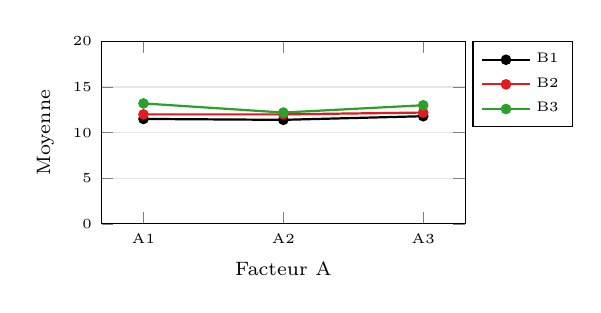
\begin{tikzpicture}
\begin{axis}[moyennes]
  \addplot[lB1] coordinates {(1,11.5) (2,11.4) (3,11.8)};
  \addplot[lB2] coordinates {(1,12.0) (2,12.0) (3,12.2)};
  \addplot[lB3] coordinates {(1,13.2) (2,12.2) (3,13.0)};
  \legend{B1, B2, B3}
\end{axis}
\end{tikzpicture}

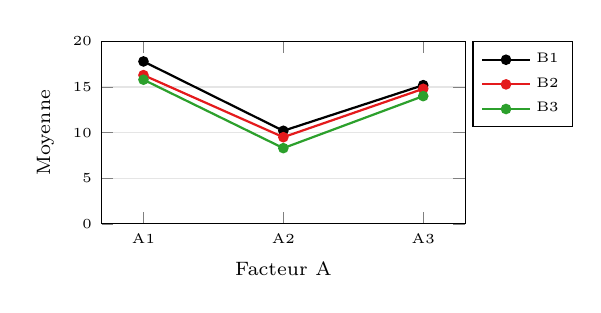
\begin{tikzpicture}
\begin{axis}[moyennes]
  \addplot[lB1] coordinates {(1,17.8) (2,10.2) (3,15.2)};
  \addplot[lB2] coordinates {(1,16.3) (2,9.5) (3,14.8)};
  \addplot[lB3] coordinates {(1,15.8) (2,8.3) (3,14.0)};
  \legend{B1, B2, B3}
\end{axis}
\end{tikzpicture}
\end{column}
\begin{column}{0.35\textwidth}
\vspace{7mm}
\begin{itemize}
  \item Interaction?
  \item Effet de A?
  \item Effet de B?
\end{itemize}
\vspace{1.4cm}
\begin{itemize}
  \item Interaction?
  \item Effet de A?
  \item Effet de B?
\end{itemize}
\end{column}
\end{columns}

\end{frame}

\begin{frame}[t]{Exercice (suite)}

\begin{columns}[T]
\begin{column}{0.62\textwidth}
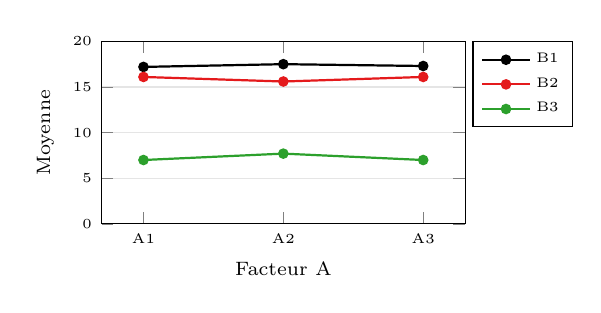
\begin{tikzpicture}
\begin{axis}[moyennes]
  \addplot[lB1] coordinates {(1,17.2) (2,17.5) (3,17.3)};
  \addplot[lB2] coordinates {(1,16.1) (2,15.6) (3,16.1)};
  \addplot[lB3] coordinates {(1,7.0) (2,7.7) (3,7.0)};
  \legend{B1, B2, B3}
\end{axis}
\end{tikzpicture}

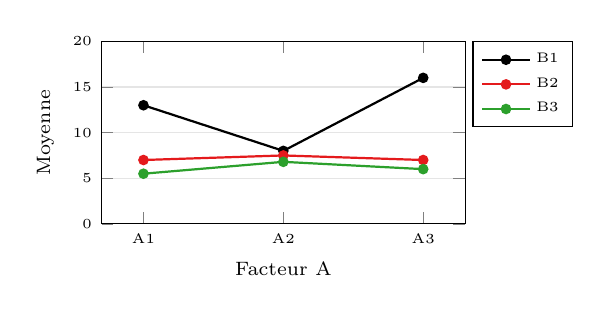
\begin{tikzpicture}
\begin{axis}[moyennes]
  \addplot[lB1] coordinates {(1,13.0) (2,8.0) (3,16.0)};
  \addplot[lB2] coordinates {(1,7.0) (2,7.5) (3,7.0)};
  \addplot[lB3] coordinates {(1,5.5) (2,6.8) (3,6.0)};
  \legend{B1, B2, B3}
\end{axis}
\end{tikzpicture}
\end{column}
\begin{column}{0.35\textwidth}
\vspace{7mm}
\begin{itemize}
  \item Interaction?
  \item Effet de A?
  \item Effet de B?
\end{itemize}
\vspace{1.4cm}
\begin{itemize}
  \item Interaction?
  \item Effet de A?
  \item Effet de B?
\end{itemize}
\end{column}
\end{columns}

\end{frame}

\begin{frame}[t]{Exemple 2: durée de vie des batteries}

On s'intéresse à l'effet du \alert{type de matériau} et de la \alert{température}
de confection (en \textdegree F) sur la \alert{durée de vie} de batteries (en heures).
On teste $n=4$ batteries à chacune des 9 combinaisons possibles de matériaux
et de températures ($a=b=3$).

\begin{center}
\small
\renewcommand{\arraystretch}{1.0}
\begin{tabular}{c|cc|cc|cc}
\toprule
 & \multicolumn{6}{c}{Température}\\
Matériau & \multicolumn{2}{c|}{15\,\textdegree F} & \multicolumn{2}{c|}{70\,\textdegree F}
 & \multicolumn{2}{c}{125\,\textdegree F}\\
\midrule
\multirow{2}{*}{1} & 130 & 155 & 34 & 40 & 20 & 70\\
                   & 74  & 180 & 80 & 75 & 82 & 58\\
\midrule
\multirow{2}{*}{2} & 150 & 188 & 126 & 122 & 25 & 70\\
                   & 159 & 126 & 106 & 115 & 58 & 45\\
\midrule
\multirow{2}{*}{3} & 138 & 110 & 174 & 120 & 96 & 104\\
                   & 168 & 160 & 150 & 139 & 82 & 60\\
\bottomrule
\end{tabular}
\end{center}

\end{frame}

\begin{frame}[t]{Graphique des moyennes}

\begin{center}
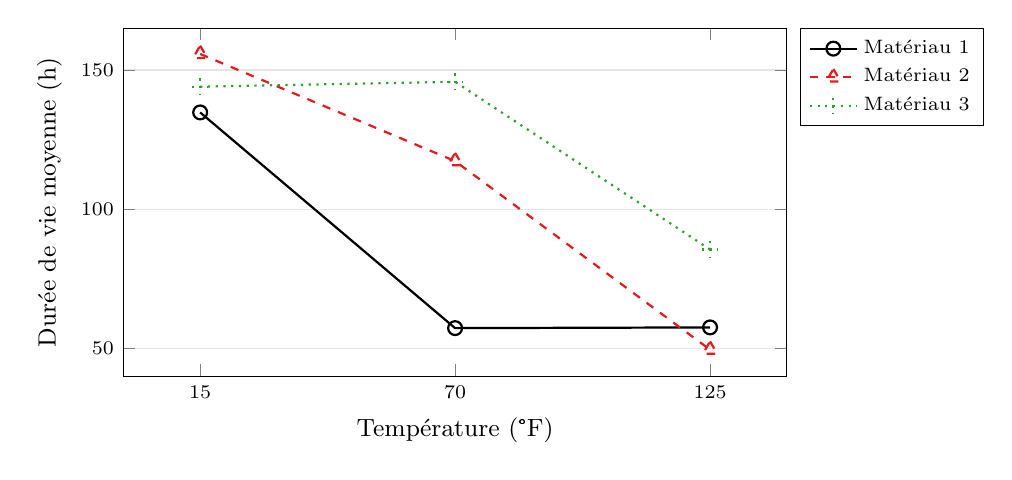
\begin{tikzpicture}
\begin{axis}[width=10cm, height=6cm, xmin=0.7, xmax=3.3, ymin=40, ymax=165,
  xtick={1,2,3}, xticklabels={15, 70, 125},
  xlabel={Température (\textdegree F)}, ylabel={Durée de vie moyenne (h)},
  tick label style={font=\scriptsize}, label style={font=\small},
  legend style={font=\scriptsize, at={(1.02,1)}, anchor=north west},
  legend cell align=left, ymajorgrids, grid style={black!10}]
  \addplot[niv1, thick, mark=o, mark size=2.5pt] coordinates {(1,134.75) (2,57.25) (3,57.5)};
  \addplot[niv2, thick, dashed, mark=triangle, mark size=3pt] coordinates {(1,155.75) (2,117.25) (3,49.5)};
  \addplot[niv3, thick, dotted, mark=+, mark size=3pt] coordinates {(1,144) (2,145.75) (3,85.5)};
  \legend{Matériau 1, Matériau 2, Matériau 3}
\end{axis}
\end{tikzpicture}
\end{center}

\end{frame}

%-------------------------------------------------------------------------------
\section{Analyse de la variance}
%-------------------------------------------------------------------------------

\begin{frame}[t]{Décomposition de la variabilité observée}

\small
\begin{align*}
\underbrace{\sum_{i=1}^{a}\sum_{j=1}^{b}\sum_{k=1}^{n}(Y_{ijk}-\overline{Y}_{\bullet\bullet\bullet})^2}_{SS_T}
&= \underbrace{bn\sum_{i=1}^{a}(\overline{Y}_{i\bullet\bullet}-\overline{Y}_{\bullet\bullet\bullet})^2}_{SS_A}
 + \underbrace{an\sum_{j=1}^{b}(\overline{Y}_{\bullet j\bullet}-\overline{Y}_{\bullet\bullet\bullet})^2}_{SS_B}\\
&\quad + \underbrace{n\sum_{i=1}^{a}\sum_{j=1}^{b}(\overline{Y}_{ij\bullet}-\overline{Y}_{i\bullet\bullet}
   -\overline{Y}_{\bullet j\bullet}+\overline{Y}_{\bullet\bullet\bullet})^2}_{SS_{AB}}
 + \underbrace{\sum_{i=1}^{a}\sum_{j=1}^{b}\sum_{k=1}^{n}(Y_{ijk}-\overline{Y}_{ij\bullet})^2}_{SS_E}
\end{align*}

où $SS_T$ est la variabilité \alert{totale}, $SS_A$ et $SS_B$ sont les variabilités
dues aux facteurs A et B, $SS_{AB}$ est la variabilité due à l'\alert{interaction}
entre A et B, et $SS_E$ est la variabilité due à l'\alert{erreur}.

\end{frame}

\begin{frame}[t]{Table d'analyse de la variance}

\begin{center}
\scriptsize
\renewcommand{\arraystretch}{2.1}
\begin{tabular}{llllll}
\toprule
Source & S.C. & d.l. & Carré moyen & $F_0$ & Valeur-p\\
\midrule
Facteur A & $SS_A$ & $a-1$ & $MS_A=\dfrac{SS_A}{a-1}$ & $F_0^A=\dfrac{MS_A}{MS_E}$
  & $P(F_{a-1;\,ab(n-1)}>F_0^A)$\\
Facteur B & $SS_B$ & $b-1$ & $MS_B=\dfrac{SS_B}{b-1}$ & $F_0^B=\dfrac{MS_B}{MS_E}$
  & $P(F_{b-1;\,ab(n-1)}>F_0^B)$\\
Interaction & $SS_{AB}$ & $(a-1)(b-1)$ & $MS_{AB}=\dfrac{SS_{AB}}{(a-1)(b-1)}$
  & $F_0^{AB}=\dfrac{MS_{AB}}{MS_E}$ & $P(F_{(a-1)(b-1);\,ab(n-1)}>F_0^{AB})$\\
Erreur & $SS_E$ & $ab(n-1)$ & $MS_E=\dfrac{SS_E}{ab(n-1)}$ & & \\
\midrule
Totale & $SS_T$ & $abn-1$ & & & \\
\bottomrule
\end{tabular}
\end{center}

\end{frame}

\begin{frame}[fragile,t]{Exemple 2: ANOVA sur la durée de vie des batteries}

\begin{Verbatim}[fontsize=\scriptsize]
> AnovaModel.1 <- lm(Duree_vie ~ Materiau*Temperature, data=batteries)
> Anova(AnovaModel.1)
Anova Table (Type II tests)

Response: Duree_vie
                     Sum Sq Df F value       Pr(>F)
Materiau              10633  2  7.9834     0.001888 **
Temperature           39083  2 29.3438 0.0000001694 ***
Materiau:Temperature   9438  4  3.5429     0.018973 *
Residuals             17981 27
\end{Verbatim}

\medskip
\begin{itemize}\itemsep1cm
  \item Quelles conclusions pouvez-vous tirer \alert{au seuil de 1\,\%}?
  \item<2-> Quelles conclusions pouvez-vous tirer \alert{au seuil de 5\,\%}?
\end{itemize}

\end{frame}

%-------------------------------------------------------------------------------
\section{Validation des postulats du modèle}
%-------------------------------------------------------------------------------

\begin{frame}[t]{Postulats et analyse des résidus}

\begin{enumerate}\itemsep3mm
  \item \alert{Indépendance} des observations:\\
  \uncover<2->{randomisation? informations sur la collecte?}
  \item \alert{Normalité} des $\varepsilon_{ijk}$:\\
  \uncover<3->{histogramme et graphique quantile-quantile normal des résidus,
  test de Shapiro-Wilk;}
  \item \alert{Variance homogène} des $\varepsilon_{ijk}$ pour chaque combinaison de facteurs:\\
  \uncover<4->{graphique des résidus en fonction des moyennes $\overline{Y}_{ij\bullet}$
  (ou diagrammes en boîtes juxtaposés), test de Bartlett.}
\end{enumerate}

\uncover<5->{
\begin{Boite}{Résidus}
Les erreurs $\varepsilon_{ijk}$ sont estimées par les résidus
$\hat\varepsilon_{ijk}=y_{ijk}-\overline{y}_{ij\bullet}$.
\end{Boite}}

\end{frame}

\begin{frame}[fragile,t]{Exemple 2: R Commander}

\begin{itemize}\itemsep5mm
  \item Pour commander une analyse de variance à plusieurs facteurs:\\
  menu \textsf{Statistiques} $\rightarrow$ \textsf{Moyennes}
  $\rightarrow$ \textsf{ANOVA à plusieurs facteurs}.
  \item Pour ajouter les résidus au jeu de données:\\
  menu \textsf{Modèles} $\rightarrow$ \textsf{Ajouter les statistiques des
  observations aux données} (cocher \textsf{Valeurs ajustées} et \textsf{Résidus}).
\end{itemize}

\medskip
Directement en R:
\begin{Verbatim}[fontsize=\small]
modele <- lm(Duree_vie ~ Materiau*Temperature, data=batteries)
batteries$residus  <- residuals(modele)
batteries$ajustees <- fitted(modele)
\end{Verbatim}

\end{frame}

\begin{frame}[fragile,t]{Exemple 2: analyse des résidus (normalité)}

\begin{center}
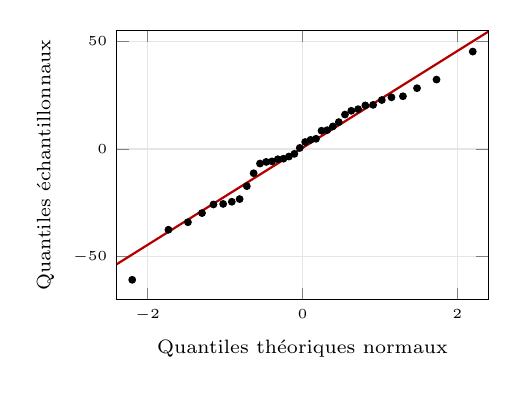
\begin{tikzpicture}
\begin{axis}[width=6.3cm, height=5cm, xlabel={Quantiles théoriques normaux},
  ylabel={Quantiles échantillonnaux}, tick label style={font=\tiny},
  label style={font=\scriptsize}, grid=major, grid style={black!10},
  xmin=-2.4, xmax=2.4, ymin=-70, ymax=55]
  \addplot[red!70!black, thick, domain=-2.4:2.4] {0.5+22.5*x};
  \addplot[only marks, mark=*, mark size=1.2pt] coordinates {
  (-2.200,-60.75) (-1.732,-37.50) (-1.480,-34.00) (-1.298,-29.75) (-1.150,-25.75)
  (-1.025,-25.50) (-0.913,-24.50) (-0.812,-23.25) (-0.719,-17.25) (-0.631,-11.25)
  (-0.549,-6.75) (-0.469,-6.00) (-0.393,-5.75) (-0.319,-4.75) (-0.246,-4.50)
  (-0.175,-3.50) (-0.105,-2.25) (-0.035,0.50) (0.035,3.25) (0.105,4.25)
  (0.175,4.75) (0.246,8.50) (0.319,8.75) (0.393,10.50) (0.469,12.50)
  (0.549,16.00) (0.631,17.75) (0.719,18.50) (0.812,20.25) (0.913,20.50)
  (1.025,22.75) (1.150,24.00) (1.298,24.50) (1.480,28.25) (1.732,32.25) (2.200,45.25)};
\end{axis}
\end{tikzpicture}
\hspace{2mm}
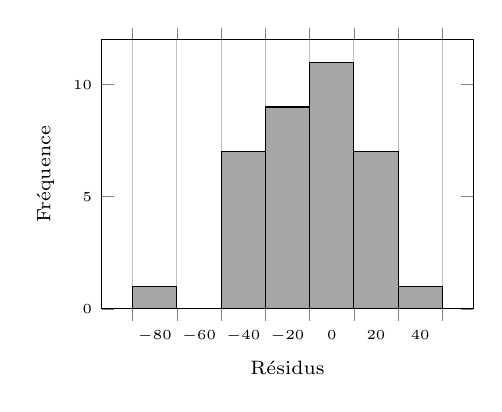
\begin{tikzpicture}
\begin{axis}[width=6.3cm, height=5cm, ybar interval, xlabel={Résidus},
  ylabel={Fréquence}, tick label style={font=\tiny}, label style={font=\scriptsize},
  ymin=0, ymax=12, xtick={-80,-60,...,60}]
  \addplot[fill=black!35, draw=black] coordinates
    {(-80,1) (-60,0) (-40,7) (-20,9) (0,11) (20,7) (40,1) (60,0)};
\end{axis}
\end{tikzpicture}
\end{center}

\begin{Verbatim}[fontsize=\scriptsize]
        Shapiro-Wilk normality test
data:  residuals.AnovaModel.1
W = 0.9777, p-value = 0.6672
\end{Verbatim}

\end{frame}

\begin{frame}[fragile,t]{Exemple 2: analyse des résidus (égalité des variances)}

\begin{center}
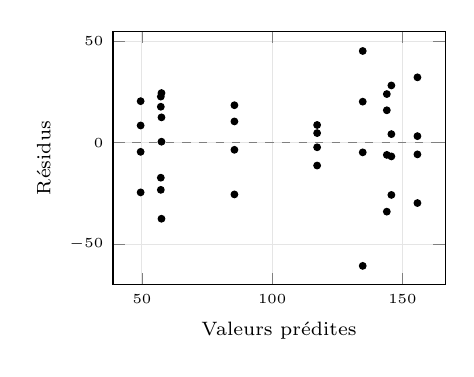
\begin{tikzpicture}
\begin{axis}[width=5.8cm, height=4.8cm, xlabel={Valeurs prédites}, ylabel={Résidus},
  tick label style={font=\tiny}, label style={font=\scriptsize},
  grid=major, grid style={black!10}, ymin=-70, ymax=55]
  \draw[dashed, gray] (axis cs:40,0) -- (axis cs:165,0);
  \addplot[only marks, mark=*, mark size=1.2pt] coordinates {
  (134.75,-4.75) (134.75,20.25) (134.75,-60.75) (134.75,45.25) (57.25,-23.25)
  (57.25,-17.25) (57.25,22.75) (57.25,17.75) (57.50,-37.50) (57.50,12.50)
  (57.50,24.50) (57.50,0.50) (155.75,-5.75) (155.75,32.25) (155.75,3.25)
  (155.75,-29.75) (117.25,8.75) (117.25,4.75) (117.25,-11.25) (117.25,-2.25)
  (49.50,-24.50) (49.50,20.50) (49.50,8.50) (49.50,-4.50) (144.00,-6.00)
  (144.00,-34.00) (144.00,24.00) (144.00,16.00) (145.75,28.25) (145.75,-25.75)
  (145.75,4.25) (145.75,-6.75) (85.50,10.50) (85.50,18.50) (85.50,-3.50) (85.50,-25.50)};
\end{axis}
\end{tikzpicture}
\hspace{1mm}
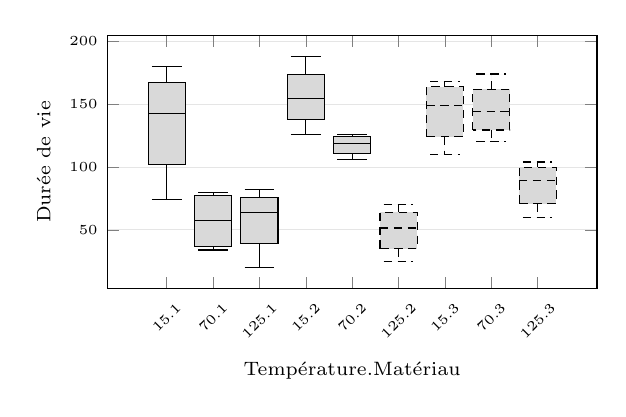
\begin{tikzpicture}
\begin{axis}[width=7.8cm, height=4.8cm, boxplot/draw direction=y,
  xtick={1,...,9}, xticklabels={15.1,70.1,125.1,15.2,70.2,125.2,15.3,70.3,125.3},
  xlabel={Température.Matériau}, ylabel={Durée de vie},
  x tick label style={font=\tiny, rotate=45}, y tick label style={font=\tiny},
  label style={font=\scriptsize}, ymajorgrids, grid style={black!10}]
  \addplot+[boxplot prepared={lower whisker=74, lower quartile=102, median=142.5, upper quartile=167.5, upper whisker=180}, black, fill=black!15] coordinates {};
  \addplot+[boxplot prepared={lower whisker=34, lower quartile=37, median=57.5, upper quartile=77.5, upper whisker=80}, black, fill=black!15] coordinates {};
  \addplot+[boxplot prepared={lower whisker=20, lower quartile=39, median=64, upper quartile=76, upper whisker=82}, black, fill=black!15] coordinates {};
  \addplot+[boxplot prepared={lower whisker=126, lower quartile=138, median=154.5, upper quartile=173.5, upper whisker=188}, black, fill=black!15] coordinates {};
  \addplot+[boxplot prepared={lower whisker=106, lower quartile=110.5, median=118.5, upper quartile=124, upper whisker=126}, black, fill=black!15] coordinates {};
  \addplot+[boxplot prepared={lower whisker=25, lower quartile=35, median=51.5, upper quartile=64, upper whisker=70}, black, fill=black!15] coordinates {};
  \addplot+[boxplot prepared={lower whisker=110, lower quartile=124, median=149, upper quartile=164, upper whisker=168}, black, fill=black!15] coordinates {};
  \addplot+[boxplot prepared={lower whisker=120, lower quartile=129.5, median=144.5, upper quartile=162, upper whisker=174}, black, fill=black!15] coordinates {};
  \addplot+[boxplot prepared={lower whisker=60, lower quartile=71, median=89, upper quartile=100, upper whisker=104}, black, fill=black!15] coordinates {};
\end{axis}
\end{tikzpicture}
\end{center}

\begin{Verbatim}[fontsize=\scriptsize]
        Bartlett test of homogeneity of variances
data:  residuals.AnovaModel.1 by interaction(Materiau, Temperature)
Bartlett's K-squared = 6.8636, df = 8, p-value = 0.5514
\end{Verbatim}

\end{frame}

\begin{frame}[t]{Réponses}

\scriptsize
\begin{itemize}\itemsep2mm
  \item \textbf{Exemple 1:} facteurs = température (A) et concentration (B);
  réponse = rendement; $a=2$, $b=3$, $n=5$.
  \item \textbf{Exercice:} (1) pas d'interaction, peu d'effet de A et de B;
  (2) pas d'interaction, effet de A, peu d'effet de B;
  (3) pas d'interaction, peu d'effet de A, effet de B;
  (4) interaction (les effets de A et B ne s'interprètent pas séparément).
  \item \textbf{Seuil de 1\,\%:} l'interaction n'est pas significative
  ($0{,}019>0{,}01$); le matériau ($p=0{,}002$) et la température ($p<0{,}001$) ont
  chacun un effet significatif sur la durée de vie moyenne.
  \item \textbf{Seuil de 5\,\%:} l'interaction est significative ($0{,}019<0{,}05$):
  l'effet de la température dépend du matériau. On interprète à l'aide du graphique
  des moyennes (p.\ ex., à 70\,\textdegree F, le matériau 3 dure beaucoup plus
  longtemps que le matériau 1).
  \item \textbf{Postulats:} Shapiro-Wilk ($p=0{,}67$) et Bartlett ($p=0{,}55$):
  pas d'évidence contre la normalité ni contre l'égalité des variances.
\end{itemize}

\end{frame}

\end{document}
